\pdfminorversion=4 % for acroread
\documentclass[aspectratio=169,t,xcolor={usenames,dvipsnames}]{beamer}
%\documentclass[t,handout,xcolor={usenames,dvipsnames}]{beamer}
\usepackage{../beamerstyle}
\usepackage{dsfont}
\usepackage{bm}
\usepackage[english]{babel}
\usepackage[utf8]{inputenc}
\usepackage{graphicx}
\usepackage{algorithm}
\usepackage[ruled,vlined,algo2e,linesnumbered]{algorithm2e}
%\usepackage[boxed,vlined]{algorithm2e}
\usepackage{hyperref}
\usepackage{booktabs}
\usepackage{mathtools}

\usepackage{amsmath,amssymb}
\usepackage{listings}
\lstset{frame=lines,framesep=3pt,numbers=left,numberblanklines=false,basicstyle=\ttfamily\small}

\usepackage{subfig}
\usepackage{multicol}
%\usepackage{appendixnumberbeamer}
%
\usepackage{tcolorbox}

\usepackage{pgfplots}
\usepackage{tikz}
\usetikzlibrary{trees} 
\usetikzlibrary{shapes.geometric}
\usetikzlibrary{positioning,shapes,shadows,arrows,calc,mindmap}
\usetikzlibrary{positioning,fadings,through}
\usetikzlibrary{decorations.pathreplacing}
\usetikzlibrary{intersections}
\usetikzlibrary{positioning,fit,calc,shadows,backgrounds}
\pgfdeclarelayer{background}
\pgfdeclarelayer{foreground}
\pgfsetlayers{background,main,foreground}
\tikzstyle{activity}=[rectangle, draw=black, rounded corners, text centered, text width=8em]
\tikzstyle{data}=[rectangle, draw=black, text centered, text width=8em]
\tikzstyle{myarrow}=[->, thick, draw=black]

% Define the layers to draw the diagram
\pgfdeclarelayer{background}
\pgfdeclarelayer{foreground}
\pgfsetlayers{background,main,foreground}

%\usepackage{listings}
%\lstset{numbers=left,
%  showstringspaces=false,
%  frame={tb},
%  captionpos=b,
%  lineskip=0pt,
%  basicstyle=\ttfamily,
%%  extendedchars=true,
%  stepnumber=1,
%  numberstyle=\small,
%  xleftmargin=1em,
%  breaklines
%}

 
\definecolor{blue}{RGB}{0, 74, 153}

\usetheme{Boadilla}
%\useinnertheme{rectangles}
\usecolortheme{whale}
\setbeamercolor{alerted text}{fg=blue}
\useoutertheme{infolines}
\setbeamertemplate{navigation symbols}{\vspace{-5pt}} % to lower the logo
\setbeamercolor{date in head/foot}{bg=white} % blue
\setbeamercolor{date in head/foot}{fg=white}
\setbeamercolor{author  in head/foot}{bg=white} %blue
\setbeamercolor{title in head/foot}{bg=white} % blue
\setbeamercolor{title}{fg=white, bg=blue}
\setbeamercolor{block title}{fg=white,bg=blue}
\setbeamercolor{block body}{bg=blue!10}
\setbeamercolor{frametitle}{fg=white, bg=blue}
\setbeamercovered{invisible}

\makeatletter
\setbeamertemplate{footline}
{
  \leavevmode%
  \hbox{%
  \begin{beamercolorbox}[wd=.333333\paperwidth,ht=2.25ex,dp=1ex,center]{author in head/foot}%
%    \usebeamerfont{author in head/foot}\insertshortauthor
  \end{beamercolorbox}%
  \begin{beamercolorbox}[wd=.333333\paperwidth,ht=2.25ex,dp=1ex,center]{title in head/foot}%
    \usebeamerfont{title in head/foot}\insertshorttitle
  \end{beamercolorbox}%
  \begin{beamercolorbox}[wd=.333333\paperwidth,ht=2.25ex,dp=1ex,right]{date in head/foot}%
    \usebeamerfont{date in head/foot}\insertshortdate{}\hspace*{2em}
%    \insertframenumber\hspace*{2ex} 
  \end{beamercolorbox}}%
  \vskip0pt%
}
\makeatother

%\pgfdeclareimage[height=1.2cm]{automl}{images/logos/automl.png}
%\pgfdeclareimage[height=1.2cm]{freiburg}{images/logos/freiburg}

%\logo{\pgfuseimage{freiburg}}

\newcommand{\comment}[1]{
	\noindent
	%\vspace{0.25cm}
	{\color{red}{\textbf{TODO:} #1}}
	%\vspace{0.25cm}
}
\renewcommand{\comment}[1]{}
\newcommand{\hide}[1]{}
\newcommand{\cemph}[2]{\emph{\textcolor{#1}{#2}}}

\newcommand{\lit}[1]{{\footnotesize\color{black!70}[#1]}}

\newcommand{\litw}[1]{{\footnotesize\color{black!20}[#1]}}


\newcommand{\myframe}[2]{\begin{frame}[c]{#1}#2\end{frame}}
\newcommand{\myframetop}[2]{\begin{frame}{#1}#2\end{frame}}
\newcommand{\myit}[1]{\begin{itemize}#1\end{itemize}}
\newcommand{\myblock}[2]{\begin{block}{#1}#2\end{block}}


\newcommand{\votepurple}[1]{\textcolor{Purple}{$\bigstar$}}
\newcommand{\voteyellow}[1]{\textcolor{Goldenrod}{$\bigstar$}}
\newcommand{\voteblue}[1]{\textcolor{RoyalBlue}{$\bigstar$}}
\newcommand{\votepink}[1]{\textcolor{Pink}{$\bigstar$}}

\newcommand{\diff}{\mathop{}\!\mathrm{d}}
\newcommand{\refstyle}[1]{{\small{\textcolor{gray}{#1}}}}
\newcommand{\hands}[0]{\includegraphics[height=1.5em]{images/hands}}
\newcommand{\transpose}[0]{{\textrm{\tiny{\sf{T}}}}}
\newcommand{\norm}{{\mathcal{N}}}
\newcommand{\cutoff}[0]{\kappa}
\newcommand{\instD}[0]{\dataset}
\newcommand{\insts}[0]{\mathcal{I}}
\newcommand{\inst}[0]{i}
\newcommand{\pcs}[0]{\mathbf{\Lambda}}
\newcommand{\bx}[0]{\conf}
\newcommand{\conf}[0]{\mathbf{\lambda}}
\newcommand{\defconf}[0]{\mathbf{\lambda}_{\text{def}}}
\newcommand{\finconf}[0]{\mathbf{\lambda}^*}
\newcommand{\incumbent}[0]{\finconf}
\newcommand{\confs}[0]{\pcs}
%\newcommand{\vlambda}[0]{\bm{\lambda}}
%\newcommand{\vLambda}[0]{\bm{\Lambda}}
\newcommand{\dataset}[0]{\mathcal{D}}
\newcommand{\datasets}[0]{\mathbf{D}}
\newcommand{\loss}[0]{\mathcal{L}}

% \renewcommand{\vec}[1]{\mathbf{#1}}
\newcommand{\hist}[0]{\mathcal{H}}
\newcommand{\param}[0]{p}
\newcommand{\algo}[0]{\mathcal{A}}
\newcommand{\algos}[0]{\mathbf{A}}
%\newcommand{\nn}[0]{N}
\newcommand{\feats}[0]{\mathcal{F}}
\newcommand{\feat}[0]{\vec{f}}
\newcommand{\cluster}[0]{\vec{h}}
\newcommand{\clusters}[0]{\vec{H}}
\newcommand{\perf}[0]{\mathbb{R}}
%\newcommand{\surro}[0]{\mathcal{S}}
\newcommand{\surro}[0]{\hat{f}}
\newcommand{\func}[0]{f}
\newcommand{\epm}[0]{\surro}
\newcommand{\portfolio}[0]{\mathcal{P}}
\newcommand{\schedule}[0]{\mathcal{S}}
\newcommand{\mdata}[0]{\dataset_{\text{meta}}}

% Deep Learning
\newcommand{\weights}[0]{\theta}
\newcommand{\metaweights}[0]{\phi}


% reinforcement learning
\newcommand{\policies}[0]{\Pi}
\newcommand{\policy}[0]{\pi}
\newcommand{\actionRL}[0]{a}
\newcommand{\stateRL}[0]{s}
\newcommand{\statesRL}[0]{\mathcal{S}}
\newcommand{\rewardRL}[0]{r}
\newcommand{\rewardfuncRL}[0]{\mathcal{R}}

\RestyleAlgo{algoruled}
\DontPrintSemicolon
\LinesNumbered
\SetAlgoVlined
\SetFuncSty{textsc}

\SetKwInOut{Input}{Input}
\SetKwInOut{Output}{Output}
\SetKw{Return}{return}

%\newcommand{\changed}[1]{{\color{red}#1}}

%\newcommand{\citeN}[1]{\citeauthor{#1}~(\citeyear{#1})}

\renewcommand{\vec}[1]{\mathbf{#1}}
\DeclareMathOperator*{\argmin}{arg\,min}
\DeclareMathOperator*{\argmax}{arg\,max}

\newcommand{\aqme}{\textit{AQME}}
\newcommand{\aslib}{\textit{ASlib}}
\newcommand{\llama}{\textit{LLAMA}}
\newcommand{\satzilla}{\textit{SATzilla}}
\newcommand{\satzillaY}[1]{\textit{SATzilla'{#1}}}
\newcommand{\snnap}{\textit{SNNAP}}
\newcommand{\claspfolioTwo}{\textit{claspfolio~2}}
\newcommand{\flexfolio}{\textit{FlexFolio}}
\newcommand{\claspfolioOne}{\textit{claspfolio~1}}
\newcommand{\isac}{\textit{ISAC}}
\newcommand{\eisac}{\textit{EISAC}}
\newcommand{\sss}{\textit{3S}}
\newcommand{\sunny}{\textit{Sunny}}
\newcommand{\ssspar}{\textit{3Spar}}
\newcommand{\cshc}{\textit{CSHC}}  
\newcommand{\cshcpar}{\textit{CSHCpar}}  
\newcommand{\measp}{\textit{ME-ASP}} 
\newcommand{\aspeed}{\textit{aspeed}}
\newcommand{\autofolio}{\textit{AutoFolio}}
\newcommand{\cedalion}{\textit{Cedalion}}
\newcommand{\fanova}{\textit{fANOVA}}
\newcommand{\sbs}{\textit{SB}}
\newcommand{\oracle}{\textit{VBS}}

% like approaches
\newcommand{\claspfoliolike}[1]{\texttt{claspfolio-#1-like}}
\newcommand{\satzillalike}[1]{\texttt{SATzilla'#1-like}}
\newcommand{\isaclike}{\texttt{ISAC-like}}
\newcommand{\ssslike}{\texttt{3S-like}}
\newcommand{\measplike}{\texttt{ME-ASP-like}}

\newcommand{\aspCoseal}{\textit{ASP-POTASSCO}}
\newcommand{\cspCoseal}{\textit{CSP-2010}}
\newcommand{\maxsatCoseal}{\textit{MAXSAT12-PMS}}
\newcommand{\premarCoseal}{\textit{PRE\-MARSHALLING}}
\newcommand{\qbfCoseal}{\textit{QBF-2011}}
\newcommand{\satallTwelveCoseal}{\textit{SAT12-ALL}}
\newcommand{\sathandTwelveCoseal}{\textit{SAT12-HAND}}
\newcommand{\satinduTwelveCoseal}{\textit{SAT12-INDU}}
\newcommand{\satrandTwelveCoseal}{\textit{SAT12-RAND}}
\newcommand{\sathandElevenCoseal}{\textit{SAT11-HAND}}
\newcommand{\satinduElevenCoseal}{\textit{SAT11-INDU}}
\newcommand{\satrandElevenCoseal}{\textit{SAT11-RAND}}
\newcommand{\proteusCoseal}{\textit{PROTEUS-2014}}

\newcommand{\irace}{\textit{I/F-race}}
\newcommand{\gga}{\textit{GGA}}
\newcommand{\smac}{\textit{SMAC}}
\newcommand{\paramils}{\textit{ParamILS}}
\newcommand{\spearmint}{\textit{Spearmint}}
\newcommand{\tpe}{\textit{TPE}}

\newcommand{\gringo}{\textit{gringo}}
\newcommand{\clasp}{\textit{clasp}}
\newcommand{\lingeling}{\textit{lingeling}}

\newcommand{\hydra}{\textit{Hydra}}

\newcommand{\plingeling}{\textit{Plingeling}}
\newcommand{\ccasat}{\textit{CCASat}}

\usepackage{pifont}
\newcommand{\itarrow}{\mbox{\Pisymbol{pzd}{229}}}
\newcommand{\ithook}{\mbox{\Pisymbol{pzd}{52}}}
\newcommand{\itcross}{\mbox{\Pisymbol{pzd}{56}}}
\newcommand{\ithand}{\mbox{\raisebox{-1pt}{\Pisymbol{pzd}{43}}}}

%\DeclareMathOperator*{\argmax}{arg\,max}

\newcommand{\ie}{{\it{}i.e.\/}}
\newcommand{\eg}{{\it{}e.g.\/}}
\newcommand{\cf}{{\it{}cf.\/}}
\newcommand{\wrt}{\mbox{w.r.t.}}
\newcommand{\vs}{{\it{}vs\/}}
\newcommand{\vsp}{{\it{}vs\/}}
\newcommand{\etc}{{\copyedit{etc.}}}
\newcommand{\etal}{{\it{}et al.\/}}

\newcommand{\pscProc}{{\bf procedure}}
\newcommand{\pscBegin}{{\bf begin}}
\newcommand{\pscEnd}{{\bf end}}
\newcommand{\pscEndIf}{{\bf endif}}
\newcommand{\pscFor}{{\bf for}}
\newcommand{\pscEach}{{\bf each}}
\newcommand{\pscThen}{{\bf then}}
\newcommand{\pscElse}{{\bf else}}
\newcommand{\pscWhile}{{\bf while}}
\newcommand{\pscIf}{{\bf if}}
\newcommand{\pscRepeat}{{\bf repeat}}
\newcommand{\pscUntil}{{\bf until}}
\newcommand{\pscWithProb}{{\bf with probability}}
\newcommand{\pscOtherwise}{{\bf otherwise}}
\newcommand{\pscDo}{{\bf do}}
\newcommand{\pscTo}{{\bf to}}
\newcommand{\pscOr}{{\bf or}}
\newcommand{\pscAnd}{{\bf and}}
\newcommand{\pscNot}{{\bf not}}
\newcommand{\pscFalse}{{\bf false}}
\newcommand{\pscEachElOf}{{\bf each element of}}
\newcommand{\pscReturn}{{\bf return}}

%\newcommand{\param}[1]{{\sl{}#1}}
\newcommand{\var}[1]{{\it{}#1}}
\newcommand{\cond}[1]{{\sf{}#1}}
%\newcommand{\state}[1]{{\sf{}#1}}
%\newcommand{\func}[1]{{\sl{}#1}}
\newcommand{\set}[1]{{\Bbb #1}}
%\newcommand{\inst}[1]{{\tt{}#1}}
\newcommand{\myurl}[1]{{\small\sf #1}}

\newcommand{\Nats}{{\Bbb N}}
\newcommand{\Reals}{{\Bbb R}}
\newcommand{\extset}[2]{\{#1 \; | \; #2\}}

\newcommand{\vbar}{$\,\;|$\hspace*{-1em}\raisebox{-0.3mm}{$\,\;\;|$}}
\newcommand{\vendbar}{\raisebox{+0.4mm}{$\,\;|$}}
\newcommand{\vend}{$\,\:\lfloor$}


\newcommand{\goleft}[2][.7]{\parbox[t]{#1\linewidth}{\strut\raggedright #2\strut}}
\newcommand{\rightimage}[2][.3]{\mbox{}\hfill\raisebox{1em-\height}[0pt][0pt]{\includegraphics[width=#1\linewidth]{#2}}\vspace*{-\baselineskip}}




\usepackage{amssymb}
\usepackage{wrapfig}
\newcommand{\argminA}{\mathop{\mathrm{argmin}}}

% FH: I created this command videotitle (and file title_slide.tex) to show a new title slide for each video without the need of any repeating boiler plate code. Please do not change this anymore.
\newcommand{\videotitle}[1]{\subtitle{#1}%%%%%%%%%%%%%%%%% Title slide -- only change title %%%%%%%%%%%%%%%
%\title{\lecturetitle}
%\subtitle{\weektitle}
%\\\vspace*{0.3cm}
% ---------------------------------------------------------------------
{
\setbeamertemplate{footline}{} % remove footer on first slide
	\frame[c]{
	\titlepage
	}
}
}

\title[AutoML: NAS]{AutoML: Neural Architecture Search (NAS)} % week title
\subtitle{Part 2: One-shot Neural Architecture Search} % video title
\author[Marius Lindauer]{Bernd Bischl \and \underline{Frank Hutter} \and Lars Kotthoff\newline \and Marius Lindauer \and Joaquin Vanschoren}
\institute{}
\date{}

\AtBeginSection[]{}

% for final handout:
\renewcommand{\videotitle}[1]{\subtitle{#1}\section{#1}%%%%%%%%%%%%%%%%% Title slide -- only change title %%%%%%%%%%%%%%%
%\title{\lecturetitle}
%\subtitle{\weektitle}
%\\\vspace*{0.3cm}
% ---------------------------------------------------------------------
{
\setbeamertemplate{footline}{} % remove footer on first slide
	\frame[c]{
	\titlepage
	}
}
}
\AtBeginSection[]{\begin{frame}{Outline}\bigskip\vfill\tableofcontents[currentsection]\end{frame}}

\begin{document}	
\maketitle

\newcommand{\lecturetitle}{Neural Architecture Search (NAS)}

%\videotitle{One-shot Neural Architecture Search}

%-------------------------------------------------
%-------------------------------------------------

%----------------------------------------------------------------------
\myframe{Convolutional Neural Fabrics \litw{\href{https://arxiv.org/pdf/1606.02492.pdf}{Saxena and Verbeek, 2017}}}{
	\centering
	\includegraphics[width=0.7\textwidth]{images/conv_fabric.png}
	
	\begin{itemize}
	\footnotesize
		\item One path from the input to the output of the lattice determines the network structure.
		\item Paths (architectures) that overlap also share the parameters.
	\end{itemize}
	
}
%----------------------------------------------------------------------

%-----------------------------------------------------------------------
\myframetop{Weight sharing and one-shot models}{

\myit{
	\item All possible architectures are subgraphs of a large supergraph (the \alert{one-shot model})
	\item This one-shot model is \alert{trained as a standard neural network} with mini-batches and stochastic optimizers.
	\item At each mini-batch iteration \alert{weights are shared} between different architectures with common edges/nodes in the supergraph
	}
	
	\centering
	\includegraphics[width=0.2\textwidth]{images/one_shot_model_1.png}\quad\quad
	\includegraphics[width=0.2\textwidth]{images/one_shot_model_2.png}\quad\quad
	\includegraphics[width=0.2\textwidth]{images/one_shot_model_3.png}

}
%----------------------------------------------------------------------

%-----------------------------------------------------------------------
%\myframetop{Basic Principle}{
%	\centering
%	\includegraphics[width=0.7\textwidth]{images/snas_oneshot.png}
%	
%	\only<1>{
%	\begin{itemize}
%	\footnotesize
%		\item The \textbf{one-shot model} is a multi-graph containing all possible DAGs
%		\myit{
%		\footnotesize
%			\item[-] Every DAG represents a single architecture $Z^{(\cdot)}$ in the search space $\mathcal{A}$.
%			\item[-] Nodes represent aggregating operations (e.g. summation, concatenation) for incoming tensors.
%			\item[-] Edges represent operations $O^i$ (in the figure: one color per operation)
%			}
%		\item The row labels in the matrix above represent a pair of nodes $(j,k)$ in the graph and the column labels the operations $O^i$. A value of $1$ means that that operaration is active in the edge connecting node $j$ to $k$.
%	\end{itemize}
%	}
%	
%	\only<2>{
%	\begin{itemize}
%	\footnotesize
%		\item The most important principle in one-shot models is \textbf{weight-sharing} between graphs.
%		\myit{
%		\footnotesize
%			\item[-] The one-shot model is trained as a normal neural network, i.e. with mini-batch training. The question is how to distinguish single architectures in the one-shot model during this training?
%			\item[-] One way is that for each sampled mini-batch also sample stochastically an architecture (DAG) and update only the parameters of that architecture.
%			\item[-] For all subsequent iterations in case a new sampled architecture has common edges (i.e. some entries in the matrices are the same) in the DAG, the weights are shared.
%			}
%	\end{itemize}
%	}
%}
%----------------------------------------------------------------------

%----------------------------------------------------------------------

\myframetop{Impact of DropPath \litw{\href{http://proceedings.mlr.press/v80/bender18a/bender18a.pdf}{Bender et al., 2018}}}{
	\centering
	
	\includegraphics[width=0.9\textwidth]{images/bender_1.png}
	
	\begin{itemize}
	%\footnotesize
		\item One other way to distinguish the single architectures in the one-shot model is as follows:
		\begin{enumerate}
			\item Train the one-shot model as a normal network without sampling any individual path (a matrix with only ones "Basic Principle" slide).
			\item Sample $K$ individual architectures after training the one-shot model and evaluate those on the validation set with the one-shot model weight.
			\item Choose the best on validation and re-train that from scratch and return the test error.
		\end{enumerate}
	\end{itemize}
	
}
%----------------------------------------------------------------------

%----------------------------------------------------------------------

\myframetop{Impact of DropPath \litw{\href{http://proceedings.mlr.press/v80/bender18a/bender18a.pdf}{Bender et al., 2018}}}{
	\centering
	
	\includegraphics[width=0.8\textwidth]{images/droppath.png}
	
    \begin{itemize}
		\item DropPath zeros out one a subset of the operations at each mini-batch training iteration with probability $p$.
		\item ScheduledDropPath starts with $p=0$ and increases that linearly throughout training until a maximum $p_{max}$ in the end.
	\end{itemize}


}
%---------------------------------------------------------------

%----------------------------------------------------------------------

\myframe{Impact of DropPath \litw{\href{http://proceedings.mlr.press/v80/bender18a/bender18a.pdf}{Bender et al., 2018}}}{
	\centering
	
    	\begin{minipage}{0.4\textwidth}
        	\begin{itemize}
				%\footnotesize
				\item If the DropPath rate is properly tuned the correlation between architectures evaluated with the one-shot weights and retrained from scratch (stand-alone models) is high.
				\item This implies that \textbf{selecting the best architecture based on the one-shot weights} is not sub-optimal.
			\end{itemize}
	    \end{minipage}
	    \hspace{1cm}
    	\begin{minipage}{0.5\textwidth}
	        \includegraphics[width=.8\textwidth]{images/bender_correlation.png}    	
    	\end{minipage}

}
%---------------------------------------------------------------

%----------------------------------------------------------------------

\myframetop{Random Search with Weight Sharing \litw{\href{https://arxiv.org/pdf/1902.07638.pdf}{Li and Talwalkar, 2020}}}{
	\centering
	
    \begin{itemize}
		\item Random Search with Weight Sharing \textbf{utilizes the one-shot model to speed up vanilla random search} as follows:
		\myit{
			\only<1>{
			\item[-] At each mini-batch iteration during the training of the one-shot model \alert{sample uniformly at random} one architecture $Z$ from the search space $\mathcal{A}$.
			\item[-] \alert{Update the parameters of the one-shot model} corresponding to only that architecture.
			\item[-] After training the one-shot model finishes, sample uniformly at random $M$ architectures and rank them based on the error on a single mini-batch from the validation set \alert{using the one-shot model parameters} (retraining from scratch is computationaly expensive).
			\item[-] Select the top $K$, where $K < M$, and evaluate those on the full validation set, again using the one-shot parameters.
			\item[-] Return the top performing architecture to \alert{retrain from scratch}.
			}
			\only<2>{
			\item[-] Works \alert{comparably to state-of-the-art NAS methods} on many benchmarks.
			}
		}
	\end{itemize}
	
	\only<2>{
	\includegraphics[width=.75\textwidth]{images/rs_ws.png}
	}
}
%---------------------------------------------------------------


%----------------------------------------------------------------------

\myframetop{Efficient Neural Architecture Search \litw{\href{https://arxiv.org/pdf/1802.03268.pdf}{Pham et al., 2018}}}{
	\centering
	
    \begin{itemize}
		\item Random Search with Weight Sharing \textbf{utilizes the one-shot model to speed up vanilla random search} as follows:
		\myit{
			\only<1>{
			\item[-] At each mini-batch iteration during the training of the one-shot model \alert{sample uniformly at random} one architecture $Z$ from the search space $\mathcal{A}$.
			\item[-] \alert{Update the parameters of the one-shot model} corresponding to only that architecture.
			\item[-] After training the one-shot model finishes, sample uniformly at random $M$ architectures and rank them based on the error on a single mini-batch from the validation set \alert{using the one-shot model parameters} (retraining from scratch is computationaly expensive).
			\item[-] Select the top $K$, where $K < M$, and evaluate those on the full validation set, again using the one-shot parameters.
			\item[-] Return the top performing architecture to \alert{retrain from scratch}.
			}
			\only<2>{
			\item[-] Works \alert{comparably to state-of-the-art NAS methods} on many benchmarks.
			}
		}
	\end{itemize}
	
	\only<2>{
	\includegraphics[width=.75\textwidth]{images/rs_ws.png}
	}
}
%---------------------------------------------------------------

%----------------------------------------------------------------------
\myframe{Questions to Answer for Yourself / Discuss with Friends}{

	\myit{
		\item Repetition:\\ \alert{What are some pros and cons of the cell search space compared to the basic one?}
\bigskip
		\item Repetition:\\ \alert{Explain the way in which level-3 motivs in the hierarchical search space use level-2 motivs.}
\medskip
		\item Repetition:\\ \alert{What are some pros and cons of the hierarchical search space compared to the other ones?}
	}	 
}
%-----------------------------------------------------------------------


\videotitle{DARTS: Differentiable Architecture Search}


%----------------------------------------------------
\myframetop{DARTS: Differentiable Architecture Search \litw{\href{https://openreview.net/forum?id=S1eYHoC5FX}{Liu et al, 2018}}}{
	\myit{
		\item Use one-shot model with continuous architecture weight $\alpha$ for each operator
\onslide<2->{
        \myit{
			\item[] $x^{(j)} = \sum_{i<j}\tilde{o}^{(i,j)}(x^{(i)}) = \sum_{i<j}\sum_{o\in\mathcal{O}}
%			\text{softmax}(\alpha)
			\frac{exp(\alpha_{o}^{(i,j)})}{\sum_{o^{\prime}\in\mathcal{O}}exp(\alpha_{o^{\prime}}^{(i,j)})}o(x^{(i)})$
%            \item[-] $o^{(i,j)} \in \argmax_{o\in\mathcal{O}}\alpha_{o}^{(i,j)}$
		}
}

		\begin{columns}
			\column{0.05\textwidth}
			\column{0.3\textwidth}
			    \centering
			    {\includegraphics[scale=0.7]{images/dartsA.pdf}}\\
			    {\scriptsize (a) Initialization}
			\column{0.3\textwidth}
\onslide<1->{
			    \centering
			    {\includegraphics[scale=0.7]{images/dartsB.pdf}}\\
			    {\scriptsize (b) Search end}
}
			\column{0.3\textwidth}
\onslide<4->{
			    \centering
			    {\includegraphics[scale=0.7]{images/dartsC.pdf}}\\
			    {\scriptsize (c) Final cell}
}
			\column{0.05\textwidth}
        \end{columns}
			
		\medskip
		\pause
\onslide<3->{
		\item By optimizing the architecture weights $\alpha$, DARTS assigns importance to each operation
		\myit{
			\item Since the $\alpha$ are continuous, we can optimize them with gradient descent
		}
}		
\medskip	
\pause
	
\vspace*{-0.2cm}
\onslide<4->{
	\item In the end, DARTS discretizes to obtain a single architecture (c)
}
	
	}
}

%----------------------------------------------------------------------

%----------------------------------------------------

\myframe{DARTS: Architecture Optimization}{

	\myit{
		\item The optimization problem (a $\rightarrow$ b) is a bi-level optimization problem:
		\begin{center}
		\footnotesize{
					\begin{tcolorbox}[width = 8cm,halign=center,valign=center]
		%		\begin{eqnarray}
					%\nonumber			
					$\text{min}_{\alpha} \mathcal{L}_{\text{\alert{val}}}(w^*(\alpha), \alert{\alpha})$\\
					%\nonumber			
					$s.t.\ w^*(\alpha) \in \text{argmin}_{w} \mathcal{L}_{\text{\alert{train}}}(\alert{w},\alpha)$
		%		\end{eqnarray}
			\end{tcolorbox}
		}
		\end{center}	
		\medskip
		\pause
		\item This is solved using alternating SGD steps on architectural parameters $\alpha$ and weights $w$ 
	}
	
	\begin{algorithm}[H]
	 %\footnotesize%
	 %create mixed ops $\tilde{o}$ parametrized by $\alpha_{o}^{(i,j)}$ for each edge $(i,j)$\\
	 \TitleOfAlgo{DARTS 1st order\vspace*{-0.3cm}\\\rule{\textwidth}{0.5pt}}

	 \While{\textit{not converged}}{
	  Update one-shot weights $\vec{w}$ by $\nabla_{\vec{w}}\mathcal{L}_{train}(\vec{w}, \vec{\alpha})$\\
	  Update architectural parameters $\alpha$ by $\nabla_{\alpha}\mathcal{L}_{valid}(\vec{w}, \vec{\alpha})$\;
	 }
	 return $\argmax_{o\in\mathcal{O}}\alpha_{o}^{(i,j)}$ for each edge $(i,j)$\;
	\end{algorithm}
	
	\medskip
	\pause
	\myit{
		\item Note: there is no theory showing that this process converges
	}

}
%----------------------------------------------------

%%%%%%%%%%%%%%%%%%%%%%%%%%%%%%%%%%%%%%%%%%%%%%%%%%%%%%%%%%%%%%%%%%%%%%%
\myframetop{Strong performance on some benchmarks}{

\begin{itemize}
    \item E.g., original CNN search space
    \myit{
    	\item 8 operations on each MixedOp
    	\item 28 MixedOps in total
    	\item $> 10^{23}$ possible architectures
    }
    \item Performance
    \myit{
    	\item $<3\%$ error on CIFAR-10 in less than 1 GPU day of search
	}
\end{itemize}

\vspace{1cm}
\centering
\includegraphics[scale=0.35]{images/darts_normal_cell.png}
\hspace{1cm}
\includegraphics[scale=0.35]{images/darts_reduction_cell.png}

}
%%%%%%%%%%%%%%%%%%%%%%%%%%%%%%%%%%%%%%%%%%%%%%%%%%%%%%%%%%%%%%%%%%%%%%%%%%%%%

%%%%%%%%%%%%%%%%%%%%%%%%%%%%%%%%%%%%%%%%%%%%%%%%%%%%%%%%%%%%%%%%%%%%%%%
\myframetop{Issues -- Non-robust behaviour}{

\myit{
	\item DARTS is very sensitive w.r.t. its own hyperparameters (e.g. one-shot learning rate, $L_2$ regularization, etc.)
    \myit{
    	\visible<2->{
    	\item[-] Tuning these hyperparameters for every new task/search space is computationally expensive
    	}
    	\visible<3->{
    	\item[-] DARTS may return degenerate architectures, e.g., cells composed with only skip connections
    	}
    }
}

%\medskip
\begin{center}
	\only<3>{
		\includegraphics[scale=0.3]{images/normal_DARTS_S3.pdf}
	}
\end{center}
\begin{minipage}{.45\textwidth}
\small
\myit{
\visible<4->{
	\item \alert{RobustDARTS} \lit{\href{https://openreview.net/forum?id=H1gDNyrKDS}{Zela et al, 2020}} -- tracks the curvature of the validation loss and stops the search early based on that
	}
}
\end{minipage}
%\hspace{.5cm}
\begin{minipage}{.45\textwidth}
\myit{
\visible<5->{
\small
	\item \alert{SmoothDARTS} \lit{\href{https://arxiv.org/pdf/2002.05283.pdf}{Chen and Hsieh, 2020}} -- applies random perturbation and adversarial training to avoid bad regions
	}
	}
\end{minipage}

\medskip

\centering
\visible<4->{
	\includegraphics[scale=0.28]{images/valid_eigenvalues_traj.pdf}
}

}
%%%%%%%%%%%%%%%%%%%%%%%%%%%%%%%%%%%%%%%%%%%%%%%%%%%%%%%%%%%%%%%%%%%%%%%%%%%%%

%%%%%%%%%%%%%%%%%%%%%%%%%%%%%%%%%%%%%%%%%%%%%%%%%%%%%%%%%%%%%%%%%%%%%%%
\myframetop{Issues -- Memory constraints}{

\vspace*{-0.15cm}
	\myit{
		\item DARTS keeps the \alert{entire one-shot model in memory}, together with its computed tensors 
    	\visible<2->{
	    	\myit{
	    	   	\item[-] This constrains the search space size and the fidelity used to train the one-shot model
		    	\item[-] \alert{Impossible} to run on large datasets as ImageNet
	    	}
		}
	}

\bigskip

\begin{minipage}{.55\textwidth}
\visible<3->{A lot of research aims to fix this issue:}

\myit{
\visible<4->{
	\item \alert{GDAS} \lit{\href{https://arxiv.org/pdf/1910.04465.pdf}{Dong et al, 2019}} -- samples from a Gumbel Softmax distribution to keep only a single architecture in memory
	}
\smallskip
\visible<5->{
	\item \alert{ProxylessNAS} \lit{\href{https://openreview.net/pdf?id=HylVB3AqYm}{Cai et al, 2019}} -- computes approximate gradients on $\alpha$ keeping only 2 edges between two nodes in memory at a time 
	}
\smallskip
\visible<6->{
	\item \alert{PC-DARTS} \lit{\href{https://arxiv.org/pdf/1907.05737.pdf}{Xu et al, 2020}} -- performs the search on a subset of the 
	%total computed 
	channels in the one-shot model
	}
}
\end{minipage}
\hspace{.5cm}
\begin{minipage}{.2\textwidth}
\visible<4->{
\includegraphics[scale=0.3]{images/gdas.png}
}
\end{minipage}

}
%%%%%%%%%%%%%%%%%%%%%%%%%%%%%%%%%%%%%%%%%%%%%%%%%%%%%%%%%%%%%%%%%%%%%%%%%%%%%


%----------------------------------------------------------------------
\myframe{Questions to Answer for Yourself / Discuss with Friends}{

	\myit{
		\item Repetition:\\ \alert{What is the main difference between DARTS and the other one-shot NAS methods we saw before?}
\bigskip
		\item Repetition:\\ \alert{How does DARTS optimize the architectural weights and one-shot weights?}
\bigskip
		\item Repetition:\\ \alert{What are DARTS' main issues and how can they be fixed?}
\medskip
		\item Discussion:\\ \alert{RobustDARTS stops the architecture optimization early, before the curvature of the validation loss becomes high. Why do you think this works? 
		\\{[Hint: think about the discretization step after the DARTS search.]}}
	}	 
}
%-----------------------------------------------------------------------

%----------------------------------------------------------------------
\myframe{NASLib: A Modular and Extendable NAS Library \litw{Zela et al., 2020}}{

	\myit{
		\item Recap: Comparing head-to-head different NAS methods is difficult due to:
		\medskip
		\myit{
			\item[-] Different codebases
			\item[-] Different search and evaluation pipelines
			\item[-] Other confounding factors, e.g. library version, etc.
		}
		\pause
		\smallskip
		\item The main purpose of \textbf{NASLib} is to circumvent these issues by:
		\myit{
			\item[-] Providing a common language to implement all NAS methods and search spaces
			\item[-] Modularizing different components of NAS optimizers, e.g. one can go from DARTS to GDAS by just a method call
			\item[-] Offering the practitioner the opportunity to easily prototype new NAS methods
		}
		}

}
%----------------------------------------------------------------------

%----------------------------------------------------------------------
\myframe{NASLib: Overview}{
	\centering
	\includegraphics[width=0.85\textwidth]{images/naslib.png}\\
	
}
%----------------------------------------------------------------------

%----------------------------------------------------------------------
\myframe{NASLib building blocks: Search Spaces}{
	\centering
	\myit{
		\item NASLib's main building block is the graph object represented as a NetworkX~\footnote{https://networkx.github.io/} graph.
		\myit{
			\item[-] This is done in order to easily manipulate the graph by adding/removing nodes/edges without dealing with the complexity of the PyTorch computational graph.
			\item[-] NetworkX offers an easy high-level way of creating complex structures, e.g. hierarchical search spaces.
			}
		\item After the NetworkX object has been built then an optimizer object interacts with it and builds the PyTorch computational graph, which can be a one-shot model or also a single architecture (depending one the optimizer, i.e. black-box optimizers will sample single architectures).
	}
	
	\includegraphics[width=0.1\textwidth]{images/naslib_space.png}
	\quad\quad
	\includegraphics[width=0.11\textwidth]{images/naslib_oneshot_model.png}	
	
}
%----------------------------------------------------------------------
%----------------------------------------------------------------------
\myframe{NASLib building blocks: Optimizers and Evaluators}{
	\centering
	\myit{
		\item NASLib supports both one-shot and black-box NAS optimizers
		\item All of them are agnostic to the search space (with NASLib's language) they run on
		\item The NAS optimizers in NASLib are also responsible for building the PyTorch computational graph by transforming the operation choices in each edge of the NetworkX graph to a:
		\myit{
				\item[-] $\texttt{MixedOp}$ -- In case the NAS optimizer is one-shot. e.g. DARTS
				\item[-] $\texttt{CategoricalOp}$ -- In case the NAS optimizer is black-box, e.g. Random Search
		}
		\item The modularized nature of these optimizers allows to transform e.g. DARTS to GDAS or PC-DARTS by just a method call.
		
		\bigskip
		\item After the one-shot model is built NASLib runs the NAS optimization routine, e.g. the bi-level loop, by using an $\texttt{Evaluator}$ object.
		\item The final returned architecture is then ran using the same object to evaluate on the test set.
	}
	
}
%----------------------------------------------------------------------
%----------------------------------------------------------------------
%\myframe{NASLib building blocks: Evaluators}{
%	\centering
%	TODO
	
%}
%----------------------------------------------------------------------
%----------------------------------------------------------------------
\myframe{Tabular benchmarks for one-shot NAS}{
	\centering
	\myit{
		\item NAS-Bench-101 \lit{\href{https://arxiv.org/abs/1902.09635}{Ying et al. 2019}} does not support one-shot NAS methods due to its graph representation
		\medskip
		\pause
		\item \alert{NAS-Bench-1Shot1} \lit{\href{https://openreview.net/forum?id=SJx9ngStPH}{Zela et al. 2020}}
		\myit{
				\item[-] Maps the graphs in NAS-Bench-101 to a representations suitable for one-shot NAS methods
				\item[-] Based on some constraints it provides 3 sub-spaces of the original NAS-Bench-101 space
				\item[-] Currently the largest one-shot NAS tabular benchmark
			}
		\smallskip
		\pause
		\item \alert{NAS-Bench-201} \lit{\href{https://openreview.net/forum?id=HJxyZkBKDr}{Dong and Yang. 2020}}
		\myit{
				\item[-] Exact same graph representation as in DARTS
				\item[-] Much smaller than NAS-Bench-101 and NAS-Bench-1Shot1
				\item[-] Every architecture in the search space evaluated on 3 image classification datasets
			}
		}
}
%----------------------------------------------------------------------
%----------------------------------------------------------------------
\myframe{NASLib case study: Results on NAS-Bench-201}{
	\centering
	\begin{minipage}{.4\textwidth}
		\myit{
			\item<1-> NAS-Bench-201 is already integrated in NASLib and we can run any one-shot optimizer on that.
			\item<2-> Or apply random perturbations to every other one-shot optimizer.
			\item<3-> Also black-box optimizers can be evaluated cheaply with a tabular benchmark.
		}	
	\end{minipage}
	\begin{minipage}{.58\textwidth}
		\centering
		\visible<1->{\includegraphics[width=0.45\textwidth]{images/nb201_1.pdf}}
		\visible<2->{\includegraphics[width=0.45\textwidth]{images/nb201_2.pdf}}\\
		\visible<3->{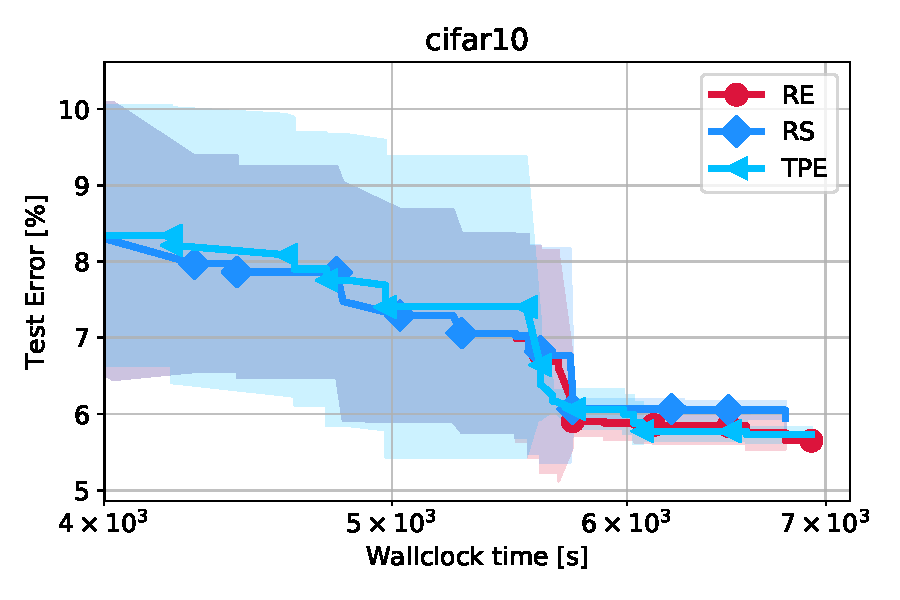
\includegraphics[width=0.55\textwidth]{images/nb201_3.pdf}}
	\end{minipage}
	
}
%----------------------------------------------------------------------




\pdfminorversion=4 % for acroread
\documentclass[aspectratio=169,t,xcolor={usenames,dvipsnames}]{beamer}
%\documentclass[t,handout,xcolor={usenames,dvipsnames}]{beamer}
\usepackage{../beamerstyle}
\usepackage{dsfont}
\usepackage{bm}
\usepackage[english]{babel}
\usepackage[utf8]{inputenc}
\usepackage{graphicx}
\usepackage{algorithm}
\usepackage[ruled,vlined,algo2e,linesnumbered]{algorithm2e}
%\usepackage[boxed,vlined]{algorithm2e}
\usepackage{hyperref}
\usepackage{booktabs}
\usepackage{mathtools}

\usepackage{amsmath,amssymb}
\usepackage{listings}
\lstset{frame=lines,framesep=3pt,numbers=left,numberblanklines=false,basicstyle=\ttfamily\small}

\usepackage{subfig}
\usepackage{multicol}
%\usepackage{appendixnumberbeamer}
%
\usepackage{tcolorbox}

\usepackage{pgfplots}
\usepackage{tikz}
\usetikzlibrary{trees} 
\usetikzlibrary{shapes.geometric}
\usetikzlibrary{positioning,shapes,shadows,arrows,calc,mindmap}
\usetikzlibrary{positioning,fadings,through}
\usetikzlibrary{decorations.pathreplacing}
\usetikzlibrary{intersections}
\usetikzlibrary{positioning,fit,calc,shadows,backgrounds}
\pgfdeclarelayer{background}
\pgfdeclarelayer{foreground}
\pgfsetlayers{background,main,foreground}
\tikzstyle{activity}=[rectangle, draw=black, rounded corners, text centered, text width=8em]
\tikzstyle{data}=[rectangle, draw=black, text centered, text width=8em]
\tikzstyle{myarrow}=[->, thick, draw=black]

% Define the layers to draw the diagram
\pgfdeclarelayer{background}
\pgfdeclarelayer{foreground}
\pgfsetlayers{background,main,foreground}

%\usepackage{listings}
%\lstset{numbers=left,
%  showstringspaces=false,
%  frame={tb},
%  captionpos=b,
%  lineskip=0pt,
%  basicstyle=\ttfamily,
%%  extendedchars=true,
%  stepnumber=1,
%  numberstyle=\small,
%  xleftmargin=1em,
%  breaklines
%}

 
\definecolor{blue}{RGB}{0, 74, 153}

\usetheme{Boadilla}
%\useinnertheme{rectangles}
\usecolortheme{whale}
\setbeamercolor{alerted text}{fg=blue}
\useoutertheme{infolines}
\setbeamertemplate{navigation symbols}{\vspace{-5pt}} % to lower the logo
\setbeamercolor{date in head/foot}{bg=white} % blue
\setbeamercolor{date in head/foot}{fg=white}
\setbeamercolor{author  in head/foot}{bg=white} %blue
\setbeamercolor{title in head/foot}{bg=white} % blue
\setbeamercolor{title}{fg=white, bg=blue}
\setbeamercolor{block title}{fg=white,bg=blue}
\setbeamercolor{block body}{bg=blue!10}
\setbeamercolor{frametitle}{fg=white, bg=blue}
\setbeamercovered{invisible}

\makeatletter
\setbeamertemplate{footline}
{
  \leavevmode%
  \hbox{%
  \begin{beamercolorbox}[wd=.333333\paperwidth,ht=2.25ex,dp=1ex,center]{author in head/foot}%
%    \usebeamerfont{author in head/foot}\insertshortauthor
  \end{beamercolorbox}%
  \begin{beamercolorbox}[wd=.333333\paperwidth,ht=2.25ex,dp=1ex,center]{title in head/foot}%
    \usebeamerfont{title in head/foot}\insertshorttitle
  \end{beamercolorbox}%
  \begin{beamercolorbox}[wd=.333333\paperwidth,ht=2.25ex,dp=1ex,right]{date in head/foot}%
    \usebeamerfont{date in head/foot}\insertshortdate{}\hspace*{2em}
%    \insertframenumber\hspace*{2ex} 
  \end{beamercolorbox}}%
  \vskip0pt%
}
\makeatother

%\pgfdeclareimage[height=1.2cm]{automl}{images/logos/automl.png}
%\pgfdeclareimage[height=1.2cm]{freiburg}{images/logos/freiburg}

%\logo{\pgfuseimage{freiburg}}

\newcommand{\comment}[1]{
	\noindent
	%\vspace{0.25cm}
	{\color{red}{\textbf{TODO:} #1}}
	%\vspace{0.25cm}
}
\renewcommand{\comment}[1]{}
\newcommand{\hide}[1]{}
\newcommand{\cemph}[2]{\emph{\textcolor{#1}{#2}}}

\newcommand{\lit}[1]{{\footnotesize\color{black!70}[#1]}}

\newcommand{\litw}[1]{{\footnotesize\color{black!20}[#1]}}


\newcommand{\myframe}[2]{\begin{frame}[c]{#1}#2\end{frame}}
\newcommand{\myframetop}[2]{\begin{frame}{#1}#2\end{frame}}
\newcommand{\myit}[1]{\begin{itemize}#1\end{itemize}}
\newcommand{\myblock}[2]{\begin{block}{#1}#2\end{block}}


\newcommand{\votepurple}[1]{\textcolor{Purple}{$\bigstar$}}
\newcommand{\voteyellow}[1]{\textcolor{Goldenrod}{$\bigstar$}}
\newcommand{\voteblue}[1]{\textcolor{RoyalBlue}{$\bigstar$}}
\newcommand{\votepink}[1]{\textcolor{Pink}{$\bigstar$}}

\newcommand{\diff}{\mathop{}\!\mathrm{d}}
\newcommand{\refstyle}[1]{{\small{\textcolor{gray}{#1}}}}
\newcommand{\hands}[0]{\includegraphics[height=1.5em]{images/hands}}
\newcommand{\transpose}[0]{{\textrm{\tiny{\sf{T}}}}}
\newcommand{\norm}{{\mathcal{N}}}
\newcommand{\cutoff}[0]{\kappa}
\newcommand{\instD}[0]{\dataset}
\newcommand{\insts}[0]{\mathcal{I}}
\newcommand{\inst}[0]{i}
\newcommand{\pcs}[0]{\mathbf{\Lambda}}
\newcommand{\bx}[0]{\conf}
\newcommand{\conf}[0]{\mathbf{\lambda}}
\newcommand{\defconf}[0]{\mathbf{\lambda}_{\text{def}}}
\newcommand{\finconf}[0]{\mathbf{\lambda}^*}
\newcommand{\incumbent}[0]{\finconf}
\newcommand{\confs}[0]{\pcs}
%\newcommand{\vlambda}[0]{\bm{\lambda}}
%\newcommand{\vLambda}[0]{\bm{\Lambda}}
\newcommand{\dataset}[0]{\mathcal{D}}
\newcommand{\datasets}[0]{\mathbf{D}}
\newcommand{\loss}[0]{\mathcal{L}}

% \renewcommand{\vec}[1]{\mathbf{#1}}
\newcommand{\hist}[0]{\mathcal{H}}
\newcommand{\param}[0]{p}
\newcommand{\algo}[0]{\mathcal{A}}
\newcommand{\algos}[0]{\mathbf{A}}
%\newcommand{\nn}[0]{N}
\newcommand{\feats}[0]{\mathcal{F}}
\newcommand{\feat}[0]{\vec{f}}
\newcommand{\cluster}[0]{\vec{h}}
\newcommand{\clusters}[0]{\vec{H}}
\newcommand{\perf}[0]{\mathbb{R}}
%\newcommand{\surro}[0]{\mathcal{S}}
\newcommand{\surro}[0]{\hat{f}}
\newcommand{\func}[0]{f}
\newcommand{\epm}[0]{\surro}
\newcommand{\portfolio}[0]{\mathcal{P}}
\newcommand{\schedule}[0]{\mathcal{S}}
\newcommand{\mdata}[0]{\dataset_{\text{meta}}}

% Deep Learning
\newcommand{\weights}[0]{\theta}
\newcommand{\metaweights}[0]{\phi}


% reinforcement learning
\newcommand{\policies}[0]{\Pi}
\newcommand{\policy}[0]{\pi}
\newcommand{\actionRL}[0]{a}
\newcommand{\stateRL}[0]{s}
\newcommand{\statesRL}[0]{\mathcal{S}}
\newcommand{\rewardRL}[0]{r}
\newcommand{\rewardfuncRL}[0]{\mathcal{R}}

\RestyleAlgo{algoruled}
\DontPrintSemicolon
\LinesNumbered
\SetAlgoVlined
\SetFuncSty{textsc}

\SetKwInOut{Input}{Input}
\SetKwInOut{Output}{Output}
\SetKw{Return}{return}

%\newcommand{\changed}[1]{{\color{red}#1}}

%\newcommand{\citeN}[1]{\citeauthor{#1}~(\citeyear{#1})}

\renewcommand{\vec}[1]{\mathbf{#1}}
\DeclareMathOperator*{\argmin}{arg\,min}
\DeclareMathOperator*{\argmax}{arg\,max}

\newcommand{\aqme}{\textit{AQME}}
\newcommand{\aslib}{\textit{ASlib}}
\newcommand{\llama}{\textit{LLAMA}}
\newcommand{\satzilla}{\textit{SATzilla}}
\newcommand{\satzillaY}[1]{\textit{SATzilla'{#1}}}
\newcommand{\snnap}{\textit{SNNAP}}
\newcommand{\claspfolioTwo}{\textit{claspfolio~2}}
\newcommand{\flexfolio}{\textit{FlexFolio}}
\newcommand{\claspfolioOne}{\textit{claspfolio~1}}
\newcommand{\isac}{\textit{ISAC}}
\newcommand{\eisac}{\textit{EISAC}}
\newcommand{\sss}{\textit{3S}}
\newcommand{\sunny}{\textit{Sunny}}
\newcommand{\ssspar}{\textit{3Spar}}
\newcommand{\cshc}{\textit{CSHC}}  
\newcommand{\cshcpar}{\textit{CSHCpar}}  
\newcommand{\measp}{\textit{ME-ASP}} 
\newcommand{\aspeed}{\textit{aspeed}}
\newcommand{\autofolio}{\textit{AutoFolio}}
\newcommand{\cedalion}{\textit{Cedalion}}
\newcommand{\fanova}{\textit{fANOVA}}
\newcommand{\sbs}{\textit{SB}}
\newcommand{\oracle}{\textit{VBS}}

% like approaches
\newcommand{\claspfoliolike}[1]{\texttt{claspfolio-#1-like}}
\newcommand{\satzillalike}[1]{\texttt{SATzilla'#1-like}}
\newcommand{\isaclike}{\texttt{ISAC-like}}
\newcommand{\ssslike}{\texttt{3S-like}}
\newcommand{\measplike}{\texttt{ME-ASP-like}}

\newcommand{\aspCoseal}{\textit{ASP-POTASSCO}}
\newcommand{\cspCoseal}{\textit{CSP-2010}}
\newcommand{\maxsatCoseal}{\textit{MAXSAT12-PMS}}
\newcommand{\premarCoseal}{\textit{PRE\-MARSHALLING}}
\newcommand{\qbfCoseal}{\textit{QBF-2011}}
\newcommand{\satallTwelveCoseal}{\textit{SAT12-ALL}}
\newcommand{\sathandTwelveCoseal}{\textit{SAT12-HAND}}
\newcommand{\satinduTwelveCoseal}{\textit{SAT12-INDU}}
\newcommand{\satrandTwelveCoseal}{\textit{SAT12-RAND}}
\newcommand{\sathandElevenCoseal}{\textit{SAT11-HAND}}
\newcommand{\satinduElevenCoseal}{\textit{SAT11-INDU}}
\newcommand{\satrandElevenCoseal}{\textit{SAT11-RAND}}
\newcommand{\proteusCoseal}{\textit{PROTEUS-2014}}

\newcommand{\irace}{\textit{I/F-race}}
\newcommand{\gga}{\textit{GGA}}
\newcommand{\smac}{\textit{SMAC}}
\newcommand{\paramils}{\textit{ParamILS}}
\newcommand{\spearmint}{\textit{Spearmint}}
\newcommand{\tpe}{\textit{TPE}}

\newcommand{\gringo}{\textit{gringo}}
\newcommand{\clasp}{\textit{clasp}}
\newcommand{\lingeling}{\textit{lingeling}}

\newcommand{\hydra}{\textit{Hydra}}

\newcommand{\plingeling}{\textit{Plingeling}}
\newcommand{\ccasat}{\textit{CCASat}}

\usepackage{pifont}
\newcommand{\itarrow}{\mbox{\Pisymbol{pzd}{229}}}
\newcommand{\ithook}{\mbox{\Pisymbol{pzd}{52}}}
\newcommand{\itcross}{\mbox{\Pisymbol{pzd}{56}}}
\newcommand{\ithand}{\mbox{\raisebox{-1pt}{\Pisymbol{pzd}{43}}}}

%\DeclareMathOperator*{\argmax}{arg\,max}

\newcommand{\ie}{{\it{}i.e.\/}}
\newcommand{\eg}{{\it{}e.g.\/}}
\newcommand{\cf}{{\it{}cf.\/}}
\newcommand{\wrt}{\mbox{w.r.t.}}
\newcommand{\vs}{{\it{}vs\/}}
\newcommand{\vsp}{{\it{}vs\/}}
\newcommand{\etc}{{\copyedit{etc.}}}
\newcommand{\etal}{{\it{}et al.\/}}

\newcommand{\pscProc}{{\bf procedure}}
\newcommand{\pscBegin}{{\bf begin}}
\newcommand{\pscEnd}{{\bf end}}
\newcommand{\pscEndIf}{{\bf endif}}
\newcommand{\pscFor}{{\bf for}}
\newcommand{\pscEach}{{\bf each}}
\newcommand{\pscThen}{{\bf then}}
\newcommand{\pscElse}{{\bf else}}
\newcommand{\pscWhile}{{\bf while}}
\newcommand{\pscIf}{{\bf if}}
\newcommand{\pscRepeat}{{\bf repeat}}
\newcommand{\pscUntil}{{\bf until}}
\newcommand{\pscWithProb}{{\bf with probability}}
\newcommand{\pscOtherwise}{{\bf otherwise}}
\newcommand{\pscDo}{{\bf do}}
\newcommand{\pscTo}{{\bf to}}
\newcommand{\pscOr}{{\bf or}}
\newcommand{\pscAnd}{{\bf and}}
\newcommand{\pscNot}{{\bf not}}
\newcommand{\pscFalse}{{\bf false}}
\newcommand{\pscEachElOf}{{\bf each element of}}
\newcommand{\pscReturn}{{\bf return}}

%\newcommand{\param}[1]{{\sl{}#1}}
\newcommand{\var}[1]{{\it{}#1}}
\newcommand{\cond}[1]{{\sf{}#1}}
%\newcommand{\state}[1]{{\sf{}#1}}
%\newcommand{\func}[1]{{\sl{}#1}}
\newcommand{\set}[1]{{\Bbb #1}}
%\newcommand{\inst}[1]{{\tt{}#1}}
\newcommand{\myurl}[1]{{\small\sf #1}}

\newcommand{\Nats}{{\Bbb N}}
\newcommand{\Reals}{{\Bbb R}}
\newcommand{\extset}[2]{\{#1 \; | \; #2\}}

\newcommand{\vbar}{$\,\;|$\hspace*{-1em}\raisebox{-0.3mm}{$\,\;\;|$}}
\newcommand{\vendbar}{\raisebox{+0.4mm}{$\,\;|$}}
\newcommand{\vend}{$\,\:\lfloor$}


\newcommand{\goleft}[2][.7]{\parbox[t]{#1\linewidth}{\strut\raggedright #2\strut}}
\newcommand{\rightimage}[2][.3]{\mbox{}\hfill\raisebox{1em-\height}[0pt][0pt]{\includegraphics[width=#1\linewidth]{#2}}\vspace*{-\baselineskip}}





\title[AutoML: NAS]{AutoML: Neural Architecture Search (NAS)} 
\subtitle{Practical Recommendations for NAS and HPO}
\author[Marius Lindauer]{Bernd Bischl \and \underline{Frank Hutter} \and Lars Kotthoff\newline \and Marius Lindauer \and Joaquin Vanschoren}
\institute{}
\date{}

\begin{document}
\maketitle

%----------------------------------------------------------------------
\myframe{Maturity of the Fields of NAS and HPO}{
	\myit{
		\item \alert{Hyperparameter optimization is a mature field}
		\myit{
			\item[-] Blackbox HPO has been researched for decades; \\ there are many software packages
			\item[-] Multi-fidelity HPO has also become quite mature
%			\item[-] Gradient-based HPO is still a nascent field
		}
\medskip
\pause
		\item \alert{Neural architecture search is still a very young field}
\pause
		\myit{
			\item[-] Blackbox is quite mature, but slow
			\item[-] Multi-fidelity NAS is also quite mature and faster
\pause
			\item[-] Meta-learning + multi-fidelity NAS is fast, but is still a very young field
\pause
\smallskip
			\item[-] Gradient-based NAS is fast, but can have failure modes with terrible performance
			\item[-] Gradient-based NAS hasn't reached the hands-off AutoML stage yet
		}
\medskip
\pause
		\item NAS is mainly used to \alert{create new architectures that many others can reuse}
		
\medskip
\pause
		\item Given a new dataset, \alert{HPO is crucial for good performance; NAS may not be necessary}
		\myit{
			\item[-] The biggest gains typically come from tuning key hyperparameters (learning rate, etc)
			\item[-] Reusing a previous achitecture often yields competitive results
		}
	}
}
%----------------------------------------------------------------------

%----------------------------------------------------------------------
\myframe{Practical Recommendations for NAS and HPO}{
	\myit{
		\item Recommendations for a new dataset
		\myit{
			\item[$\rightarrow$] Always run HPO
			\item[$\rightarrow$] Try NAS if you can 
		}
\bigskip
\pause
		\item How to combine NAS \& HPO
		\myit{
			\item[-] If the compute budget suffices, \alert{optimize them jointly}, e.g., using BOHB
			\myit{
				\item[+] Auto-PyTorch Tabular \lit{\href{https://github.com/automl/Auto-PyTorch}{Zimmer,\,Lindauer\,\& Hutter, 2020}}
				\item[+] Auto-RL \lit{\href{https://arxiv.org/pdf/1812.11951.pdf}{Runge et al. 2019}}
			}
\medskip
\pause
			\item[-] Else
			\myit{
				\item[+] If you have decent hyperparameters:\\
			\alert{run NAS, followed by HPO for fine-tuning} \lit{\href{https://arxiv.org/pdf/1905.07443.pdf}{Saikat et al. 2019}}
\smallskip
\pause
				\item[+] If you don't have decent hyperparameters: \alert{first run HPO} to get competitive	
			}
%\medskip
%\pause
%			\item[-] To improve robustness of DARTS, \\
%			tune DARTS' own hyperparameters with BOHB \lit{\href{https://openreview.net/forum?id=SJx9ngStPH}{Zela et al, 2020}}
		}
	}
}
%----------------------------------------------------------------------


%----------------------------------------------------------------------
\myframe{Case Study: NAS \& HPO in Auto-PyTorch Tabular \litw{\href{https://github.com/automl/Auto-PyTorch}{Zimmer,\,Lindauer\,\& Hutter, 2020}}}{

\begin{columns}[T]
	\column{0.29\textwidth}

\onslide<1->{
	\myit{
		\item \alert{Joint Architecture Search and Hyperparameter Optimization}
		\myit{
\onslide<2->{
			\item[-] Purely using HPO techniques: very similar methods as in \alert{Auto-sklearn 2.0}
}
\onslide<3->{
			\item[-] \alert{Multi-fidelity optimization} with \alert{BOHB}
			\item[-] \alert{Meta-learning} with \alert{task-independent recommendations}
}
\onslide<4->{
			\item[-] \alert{Ensembling} of neural nets and traditional ML models
}
}
		}
	}
	
	\column{0.29\textwidth}	
\onslide<1->{
	\includegraphics[width=\linewidth]{images/AutoPytorch-ShapedResNet.jpg}\\
}
	\column{0.42\textwidth}	
\vspace*{-0.7cm}
\onslide<1->{
	\begin{center}
	\includegraphics[width=0.9\linewidth]{images/AutoPytorch-ConfigSpace.jpg}
	\end{center}
}
\onslide<5->{
	\vspace*{-0.3cm}\hspace*{-1.1cm}
	\includegraphics[width=1.1\linewidth]{images/AutoPytorch-performance.jpg}
%	\end{center}
}


\end{columns}
}
%----------------------------------------------------------------------


%----------------------------------------------------------------------
\myframe{Case Study: NAS \& HPO in Auto-DispNet}{
	\begin{columns}[T]
		\column{0.64\textwidth}
		\myit{
			\item Problem: disparity estimation
			\myit{
				\item[-] Estimate depth from stereo images
			}
	\onslide<2->{
	\smallskip
				\item Background: U-Net
			\myit{
				\item Skip connections from similar spatial resolution to avoid loosing information
			}
	}\onslide<3->{
	\smallskip
				\item Search space for DARTS
			\myit{
				\item 3 cells: keeping spatial resolution, downsampling, 
				and \alert{new upsampling cell that supports U-Net like skip connections} 
			}
		}
	\smallskip
	}
	\onslide<4->{
		\myit{
			\item Both NAS and HPO improved the state of the art \lit{\href{https://arxiv.org/pdf/1905.07443.pdf}{Saikat et al. 2019}}:
			\myit{
				\item End-point-error (EPE) on Sintel dataset: \alert{2.36 $\rightarrow$ 2.14 (by DARTS)}
				\item Subsequent HPO: \alert{2.14 $\rightarrow$ 1.94 (by BOHB)}
			}
		}
	}

		\column{0.35\textwidth}
		\centering
		\includegraphics[width=\linewidth]{images/disparity_estimation}\\
\bigskip
\bigskip
\onslide<2->
		\includegraphics[width=\linewidth]{images/u-net-architecture}	 
	\end{columns}	
}
%----------------------------------------------------------------------

%----------------------------------------------------------------------
%\myframe{Case Study Details (Auto-DispNet)}{
%	\myit{
%		\item Very important: \alert{warmstarting} of the network weights
%		\myit{
%			\item First half of the training epochs: \\
%			keep one-shot architecture weights fixed to the uniform distribution
%			\item Only afterwards: \\
%			DARTS' alternating updates of weights and architectural parameters
%		}
%\bigskip
%		\item Without warmstarting:\\
%		\alert{DARTS found cells with only parameterless operations}
%	}	
%}
%----------------------------------------------------------------------



%----------------------------------------------------------------------
\myframe{Questions to Answer for Yourself / Discuss with Friends}{

	\myit{
		\item Repetition:\\ \alert{If you want to use both HPO and NAS for your problem, how could you proceed?}
\medskip
		\item Discussion:\\ \alert{Think of a problem of your particular interest. For that problem, which approach would you use to combine HPO and NAS, and why?}
	}	 
}
%-----------------------------------------------------------------------

%----------------------------------------------------------------------
%\myframe{Learning Goals}{
%
%	After this week's videos on HPO and NAS, you should be able to \ldots
%	
%	\begin{itemize}
%		\item describe \alert{several ways of speeding up over blackbox NAS}  %(except via meta-learning)
%		\item describe \alert{several ways of speeding up over blackbox NAS}  %(except via meta-learning)
%		\myit{
%			\item define \alert{network morphisms} \& \alert{explain how to use them to speed up NAS}
%			\item explain various \alert{multi-fidelity Bayesian optimization methods}
%		}
%		\item discuss \alert{when and how to use NAS and HPO in practice} 
%		\item describe \alert{failure modes of DARTS}
%	\end{itemize}
%}

\end{document}

\pdfminorversion=4 % for acroread
\documentclass[aspectratio=169,t,xcolor={usenames,dvipsnames}]{beamer}
%\documentclass[t,handout,xcolor={usenames,dvipsnames}]{beamer}
\usepackage{../beamerstyle}
\usepackage{dsfont}
\usepackage{bm}
\usepackage[english]{babel}
\usepackage[utf8]{inputenc}
\usepackage{graphicx}
\usepackage{algorithm}
\usepackage[ruled,vlined,algo2e,linesnumbered]{algorithm2e}
%\usepackage[boxed,vlined]{algorithm2e}
\usepackage{hyperref}
\usepackage{booktabs}
\usepackage{mathtools}

\usepackage{amsmath,amssymb}
\usepackage{listings}
\lstset{frame=lines,framesep=3pt,numbers=left,numberblanklines=false,basicstyle=\ttfamily\small}

\usepackage{subfig}
\usepackage{multicol}
%\usepackage{appendixnumberbeamer}
%
\usepackage{tcolorbox}

\usepackage{pgfplots}
\usepackage{tikz}
\usetikzlibrary{trees} 
\usetikzlibrary{shapes.geometric}
\usetikzlibrary{positioning,shapes,shadows,arrows,calc,mindmap}
\usetikzlibrary{positioning,fadings,through}
\usetikzlibrary{decorations.pathreplacing}
\usetikzlibrary{intersections}
\usetikzlibrary{positioning,fit,calc,shadows,backgrounds}
\pgfdeclarelayer{background}
\pgfdeclarelayer{foreground}
\pgfsetlayers{background,main,foreground}
\tikzstyle{activity}=[rectangle, draw=black, rounded corners, text centered, text width=8em]
\tikzstyle{data}=[rectangle, draw=black, text centered, text width=8em]
\tikzstyle{myarrow}=[->, thick, draw=black]

% Define the layers to draw the diagram
\pgfdeclarelayer{background}
\pgfdeclarelayer{foreground}
\pgfsetlayers{background,main,foreground}

%\usepackage{listings}
%\lstset{numbers=left,
%  showstringspaces=false,
%  frame={tb},
%  captionpos=b,
%  lineskip=0pt,
%  basicstyle=\ttfamily,
%%  extendedchars=true,
%  stepnumber=1,
%  numberstyle=\small,
%  xleftmargin=1em,
%  breaklines
%}

 
\definecolor{blue}{RGB}{0, 74, 153}

\usetheme{Boadilla}
%\useinnertheme{rectangles}
\usecolortheme{whale}
\setbeamercolor{alerted text}{fg=blue}
\useoutertheme{infolines}
\setbeamertemplate{navigation symbols}{\vspace{-5pt}} % to lower the logo
\setbeamercolor{date in head/foot}{bg=white} % blue
\setbeamercolor{date in head/foot}{fg=white}
\setbeamercolor{author  in head/foot}{bg=white} %blue
\setbeamercolor{title in head/foot}{bg=white} % blue
\setbeamercolor{title}{fg=white, bg=blue}
\setbeamercolor{block title}{fg=white,bg=blue}
\setbeamercolor{block body}{bg=blue!10}
\setbeamercolor{frametitle}{fg=white, bg=blue}
\setbeamercovered{invisible}

\makeatletter
\setbeamertemplate{footline}
{
  \leavevmode%
  \hbox{%
  \begin{beamercolorbox}[wd=.333333\paperwidth,ht=2.25ex,dp=1ex,center]{author in head/foot}%
%    \usebeamerfont{author in head/foot}\insertshortauthor
  \end{beamercolorbox}%
  \begin{beamercolorbox}[wd=.333333\paperwidth,ht=2.25ex,dp=1ex,center]{title in head/foot}%
    \usebeamerfont{title in head/foot}\insertshorttitle
  \end{beamercolorbox}%
  \begin{beamercolorbox}[wd=.333333\paperwidth,ht=2.25ex,dp=1ex,right]{date in head/foot}%
    \usebeamerfont{date in head/foot}\insertshortdate{}\hspace*{2em}
%    \insertframenumber\hspace*{2ex} 
  \end{beamercolorbox}}%
  \vskip0pt%
}
\makeatother

%\pgfdeclareimage[height=1.2cm]{automl}{images/logos/automl.png}
%\pgfdeclareimage[height=1.2cm]{freiburg}{images/logos/freiburg}

%\logo{\pgfuseimage{freiburg}}

\newcommand{\comment}[1]{
	\noindent
	%\vspace{0.25cm}
	{\color{red}{\textbf{TODO:} #1}}
	%\vspace{0.25cm}
}
\renewcommand{\comment}[1]{}
\newcommand{\hide}[1]{}
\newcommand{\cemph}[2]{\emph{\textcolor{#1}{#2}}}

\newcommand{\lit}[1]{{\footnotesize\color{black!70}[#1]}}

\newcommand{\litw}[1]{{\footnotesize\color{black!20}[#1]}}


\newcommand{\myframe}[2]{\begin{frame}[c]{#1}#2\end{frame}}
\newcommand{\myframetop}[2]{\begin{frame}{#1}#2\end{frame}}
\newcommand{\myit}[1]{\begin{itemize}#1\end{itemize}}
\newcommand{\myblock}[2]{\begin{block}{#1}#2\end{block}}


\newcommand{\votepurple}[1]{\textcolor{Purple}{$\bigstar$}}
\newcommand{\voteyellow}[1]{\textcolor{Goldenrod}{$\bigstar$}}
\newcommand{\voteblue}[1]{\textcolor{RoyalBlue}{$\bigstar$}}
\newcommand{\votepink}[1]{\textcolor{Pink}{$\bigstar$}}

\newcommand{\diff}{\mathop{}\!\mathrm{d}}
\newcommand{\refstyle}[1]{{\small{\textcolor{gray}{#1}}}}
\newcommand{\hands}[0]{\includegraphics[height=1.5em]{images/hands}}
\newcommand{\transpose}[0]{{\textrm{\tiny{\sf{T}}}}}
\newcommand{\norm}{{\mathcal{N}}}
\newcommand{\cutoff}[0]{\kappa}
\newcommand{\instD}[0]{\dataset}
\newcommand{\insts}[0]{\mathcal{I}}
\newcommand{\inst}[0]{i}
\newcommand{\pcs}[0]{\mathbf{\Lambda}}
\newcommand{\bx}[0]{\conf}
\newcommand{\conf}[0]{\mathbf{\lambda}}
\newcommand{\defconf}[0]{\mathbf{\lambda}_{\text{def}}}
\newcommand{\finconf}[0]{\mathbf{\lambda}^*}
\newcommand{\incumbent}[0]{\finconf}
\newcommand{\confs}[0]{\pcs}
%\newcommand{\vlambda}[0]{\bm{\lambda}}
%\newcommand{\vLambda}[0]{\bm{\Lambda}}
\newcommand{\dataset}[0]{\mathcal{D}}
\newcommand{\datasets}[0]{\mathbf{D}}
\newcommand{\loss}[0]{\mathcal{L}}

% \renewcommand{\vec}[1]{\mathbf{#1}}
\newcommand{\hist}[0]{\mathcal{H}}
\newcommand{\param}[0]{p}
\newcommand{\algo}[0]{\mathcal{A}}
\newcommand{\algos}[0]{\mathbf{A}}
%\newcommand{\nn}[0]{N}
\newcommand{\feats}[0]{\mathcal{F}}
\newcommand{\feat}[0]{\vec{f}}
\newcommand{\cluster}[0]{\vec{h}}
\newcommand{\clusters}[0]{\vec{H}}
\newcommand{\perf}[0]{\mathbb{R}}
%\newcommand{\surro}[0]{\mathcal{S}}
\newcommand{\surro}[0]{\hat{f}}
\newcommand{\func}[0]{f}
\newcommand{\epm}[0]{\surro}
\newcommand{\portfolio}[0]{\mathcal{P}}
\newcommand{\schedule}[0]{\mathcal{S}}
\newcommand{\mdata}[0]{\dataset_{\text{meta}}}

% Deep Learning
\newcommand{\weights}[0]{\theta}
\newcommand{\metaweights}[0]{\phi}


% reinforcement learning
\newcommand{\policies}[0]{\Pi}
\newcommand{\policy}[0]{\pi}
\newcommand{\actionRL}[0]{a}
\newcommand{\stateRL}[0]{s}
\newcommand{\statesRL}[0]{\mathcal{S}}
\newcommand{\rewardRL}[0]{r}
\newcommand{\rewardfuncRL}[0]{\mathcal{R}}

\RestyleAlgo{algoruled}
\DontPrintSemicolon
\LinesNumbered
\SetAlgoVlined
\SetFuncSty{textsc}

\SetKwInOut{Input}{Input}
\SetKwInOut{Output}{Output}
\SetKw{Return}{return}

%\newcommand{\changed}[1]{{\color{red}#1}}

%\newcommand{\citeN}[1]{\citeauthor{#1}~(\citeyear{#1})}

\renewcommand{\vec}[1]{\mathbf{#1}}
\DeclareMathOperator*{\argmin}{arg\,min}
\DeclareMathOperator*{\argmax}{arg\,max}

\newcommand{\aqme}{\textit{AQME}}
\newcommand{\aslib}{\textit{ASlib}}
\newcommand{\llama}{\textit{LLAMA}}
\newcommand{\satzilla}{\textit{SATzilla}}
\newcommand{\satzillaY}[1]{\textit{SATzilla'{#1}}}
\newcommand{\snnap}{\textit{SNNAP}}
\newcommand{\claspfolioTwo}{\textit{claspfolio~2}}
\newcommand{\flexfolio}{\textit{FlexFolio}}
\newcommand{\claspfolioOne}{\textit{claspfolio~1}}
\newcommand{\isac}{\textit{ISAC}}
\newcommand{\eisac}{\textit{EISAC}}
\newcommand{\sss}{\textit{3S}}
\newcommand{\sunny}{\textit{Sunny}}
\newcommand{\ssspar}{\textit{3Spar}}
\newcommand{\cshc}{\textit{CSHC}}  
\newcommand{\cshcpar}{\textit{CSHCpar}}  
\newcommand{\measp}{\textit{ME-ASP}} 
\newcommand{\aspeed}{\textit{aspeed}}
\newcommand{\autofolio}{\textit{AutoFolio}}
\newcommand{\cedalion}{\textit{Cedalion}}
\newcommand{\fanova}{\textit{fANOVA}}
\newcommand{\sbs}{\textit{SB}}
\newcommand{\oracle}{\textit{VBS}}

% like approaches
\newcommand{\claspfoliolike}[1]{\texttt{claspfolio-#1-like}}
\newcommand{\satzillalike}[1]{\texttt{SATzilla'#1-like}}
\newcommand{\isaclike}{\texttt{ISAC-like}}
\newcommand{\ssslike}{\texttt{3S-like}}
\newcommand{\measplike}{\texttt{ME-ASP-like}}

\newcommand{\aspCoseal}{\textit{ASP-POTASSCO}}
\newcommand{\cspCoseal}{\textit{CSP-2010}}
\newcommand{\maxsatCoseal}{\textit{MAXSAT12-PMS}}
\newcommand{\premarCoseal}{\textit{PRE\-MARSHALLING}}
\newcommand{\qbfCoseal}{\textit{QBF-2011}}
\newcommand{\satallTwelveCoseal}{\textit{SAT12-ALL}}
\newcommand{\sathandTwelveCoseal}{\textit{SAT12-HAND}}
\newcommand{\satinduTwelveCoseal}{\textit{SAT12-INDU}}
\newcommand{\satrandTwelveCoseal}{\textit{SAT12-RAND}}
\newcommand{\sathandElevenCoseal}{\textit{SAT11-HAND}}
\newcommand{\satinduElevenCoseal}{\textit{SAT11-INDU}}
\newcommand{\satrandElevenCoseal}{\textit{SAT11-RAND}}
\newcommand{\proteusCoseal}{\textit{PROTEUS-2014}}

\newcommand{\irace}{\textit{I/F-race}}
\newcommand{\gga}{\textit{GGA}}
\newcommand{\smac}{\textit{SMAC}}
\newcommand{\paramils}{\textit{ParamILS}}
\newcommand{\spearmint}{\textit{Spearmint}}
\newcommand{\tpe}{\textit{TPE}}

\newcommand{\gringo}{\textit{gringo}}
\newcommand{\clasp}{\textit{clasp}}
\newcommand{\lingeling}{\textit{lingeling}}

\newcommand{\hydra}{\textit{Hydra}}

\newcommand{\plingeling}{\textit{Plingeling}}
\newcommand{\ccasat}{\textit{CCASat}}

\usepackage{pifont}
\newcommand{\itarrow}{\mbox{\Pisymbol{pzd}{229}}}
\newcommand{\ithook}{\mbox{\Pisymbol{pzd}{52}}}
\newcommand{\itcross}{\mbox{\Pisymbol{pzd}{56}}}
\newcommand{\ithand}{\mbox{\raisebox{-1pt}{\Pisymbol{pzd}{43}}}}

%\DeclareMathOperator*{\argmax}{arg\,max}

\newcommand{\ie}{{\it{}i.e.\/}}
\newcommand{\eg}{{\it{}e.g.\/}}
\newcommand{\cf}{{\it{}cf.\/}}
\newcommand{\wrt}{\mbox{w.r.t.}}
\newcommand{\vs}{{\it{}vs\/}}
\newcommand{\vsp}{{\it{}vs\/}}
\newcommand{\etc}{{\copyedit{etc.}}}
\newcommand{\etal}{{\it{}et al.\/}}

\newcommand{\pscProc}{{\bf procedure}}
\newcommand{\pscBegin}{{\bf begin}}
\newcommand{\pscEnd}{{\bf end}}
\newcommand{\pscEndIf}{{\bf endif}}
\newcommand{\pscFor}{{\bf for}}
\newcommand{\pscEach}{{\bf each}}
\newcommand{\pscThen}{{\bf then}}
\newcommand{\pscElse}{{\bf else}}
\newcommand{\pscWhile}{{\bf while}}
\newcommand{\pscIf}{{\bf if}}
\newcommand{\pscRepeat}{{\bf repeat}}
\newcommand{\pscUntil}{{\bf until}}
\newcommand{\pscWithProb}{{\bf with probability}}
\newcommand{\pscOtherwise}{{\bf otherwise}}
\newcommand{\pscDo}{{\bf do}}
\newcommand{\pscTo}{{\bf to}}
\newcommand{\pscOr}{{\bf or}}
\newcommand{\pscAnd}{{\bf and}}
\newcommand{\pscNot}{{\bf not}}
\newcommand{\pscFalse}{{\bf false}}
\newcommand{\pscEachElOf}{{\bf each element of}}
\newcommand{\pscReturn}{{\bf return}}

%\newcommand{\param}[1]{{\sl{}#1}}
\newcommand{\var}[1]{{\it{}#1}}
\newcommand{\cond}[1]{{\sf{}#1}}
%\newcommand{\state}[1]{{\sf{}#1}}
%\newcommand{\func}[1]{{\sl{}#1}}
\newcommand{\set}[1]{{\Bbb #1}}
%\newcommand{\inst}[1]{{\tt{}#1}}
\newcommand{\myurl}[1]{{\small\sf #1}}

\newcommand{\Nats}{{\Bbb N}}
\newcommand{\Reals}{{\Bbb R}}
\newcommand{\extset}[2]{\{#1 \; | \; #2\}}

\newcommand{\vbar}{$\,\;|$\hspace*{-1em}\raisebox{-0.3mm}{$\,\;\;|$}}
\newcommand{\vendbar}{\raisebox{+0.4mm}{$\,\;|$}}
\newcommand{\vend}{$\,\:\lfloor$}


\newcommand{\goleft}[2][.7]{\parbox[t]{#1\linewidth}{\strut\raggedright #2\strut}}
\newcommand{\rightimage}[2][.3]{\mbox{}\hfill\raisebox{1em-\height}[0pt][0pt]{\includegraphics[width=#1\linewidth]{#2}}\vspace*{-\baselineskip}}





\title[AutoML: NAS]{AutoML: Neural Architecture Search (NAS)} 
\subtitle{Further Reading}
\author[Marius Lindauer]{Bernd Bischl \and \underline{Frank Hutter} \and Lars Kotthoff\newline \and Marius Lindauer \and Joaquin Vanschoren}
\institute{}
\date{}

\begin{document}
\maketitle

%\videotitle{Further Reading}
\begin{frame}[c]{Further Reading}

Survey on NAS:     \lit{\href{http://jmlr.org/papers/v20/18-598.html}{Elsken and Metzen and Hutter, 2019}}

\end{frame}
\end{document}

\end{document}
